% Created 2024-08-12 Mon 13:01
% Intended LaTeX compiler: pdflatex
\documentclass[11pt]{article}
\usepackage[utf8]{inputenc}
\usepackage[T1]{fontenc}
\usepackage{graphicx}
\usepackage{longtable}
\usepackage{wrapfig}
\usepackage{rotating}
\usepackage[normalem]{ulem}
\usepackage{amsmath}
\usepackage{amssymb}
\usepackage{capt-of}
\usepackage{hyperref}
\usepackage{minted}
\usepackage[a4paper, margin=2.5cm]{geometry}
\usepackage{minted}
\usepackage{fontspec}
\setmonofont{Iosevka}
\setminted{fontsize=\small, frame=single, bgcolor={HTML}{282c34}}
\usemintedstyle{one-dark}
\author{Baley Eccles - 652137}
\date{\textit{{[}2024-08-09 Fri 12:55]}}
\title{KME272 - Assesment 1.2}
\hypersetup{
 pdfauthor={Baley Eccles - 652137},
 pdftitle={KME272 - Assesment 1.2},
 pdfkeywords={},
 pdfsubject={},
 pdfcreator={Emacs 29.4 (Org mode 9.8)}, 
 pdflang={English}}
\begin{document}

\maketitle
\tableofcontents

\section{KME272 - Assesment 1.2}
\label{sec:org8c7a200}
\subsection{1}
\label{sec:orgd059dc5}
\subsubsection{(i)}
\label{sec:orgf77a0f1}
\[g(x)=3x^3+x-5\]
\[g'(x)=9x^2+1\]
The minimum occurs at \(1.1\)
\[g'(1.1)=9\cdot(1.1)^2+1=11.89>1\]
So the root will be found
\subsubsection{(ii)}
\label{sec:org8fede7a}
\[g(x)=\frac{-1}{k}(3x^3-kx-5)\]
\[g'(x)=\frac{-1}{k}(9x^2-k)\]
\[\lvert g'(x)\rvert >1\]
\[k<9x^2-k\]
\[x>\sqrt{\frac{2k}{9}} \textrm{ or } x<-\sqrt{\frac{2k}{9}}\]
\subsubsection{(iii)}
\label{sec:orgee7665f}
\begin{minted}[]{octave}
kValues = [6.5, 10, 18, 26];
tol = 10^(-6);
seeds = -5:0.01:5; % For octave 0.001 doesnt work it is too slow
stepsCount = zeros(length(seeds), length(kValues));
maxSteps = 250;
f = @(x, k) -1/k * (3*x^3 - k*x - 5);
for j = 1:length(kValues)
    k = kValues(j);
    for i = 1:length(seeds)
        x0 = seeds(i);
        x_n = x0;
        steps = 0;

        while true
            x_n1 = f(x_n, k);
            steps = steps + 1;
            if abs(x_n1 - x_n) < tol
                break;
            end
            if steps > maxSteps
                steps = NaN;
                break;
            end
            x_n = x_n1;
        end

        stepsCount(i, j) = steps;
    end
end

fig = figure ();
hold on;

for j = 1:length(kValues)
    plot(seeds, stepsCount(:, j), 'DisplayName', ['k = '    num2str(kValues(j))]);
end

hold off;

xlabel('Seed Points (x0)');
ylabel('Number of steps to Converge');
title('Convergence of Fixed-Point Iteration for Different k Values');
legend show;
grid on;
print('KME272-Assesment-1-2-Part1.png','-dpng','-r1000');
\end{minted}


\begin{center}
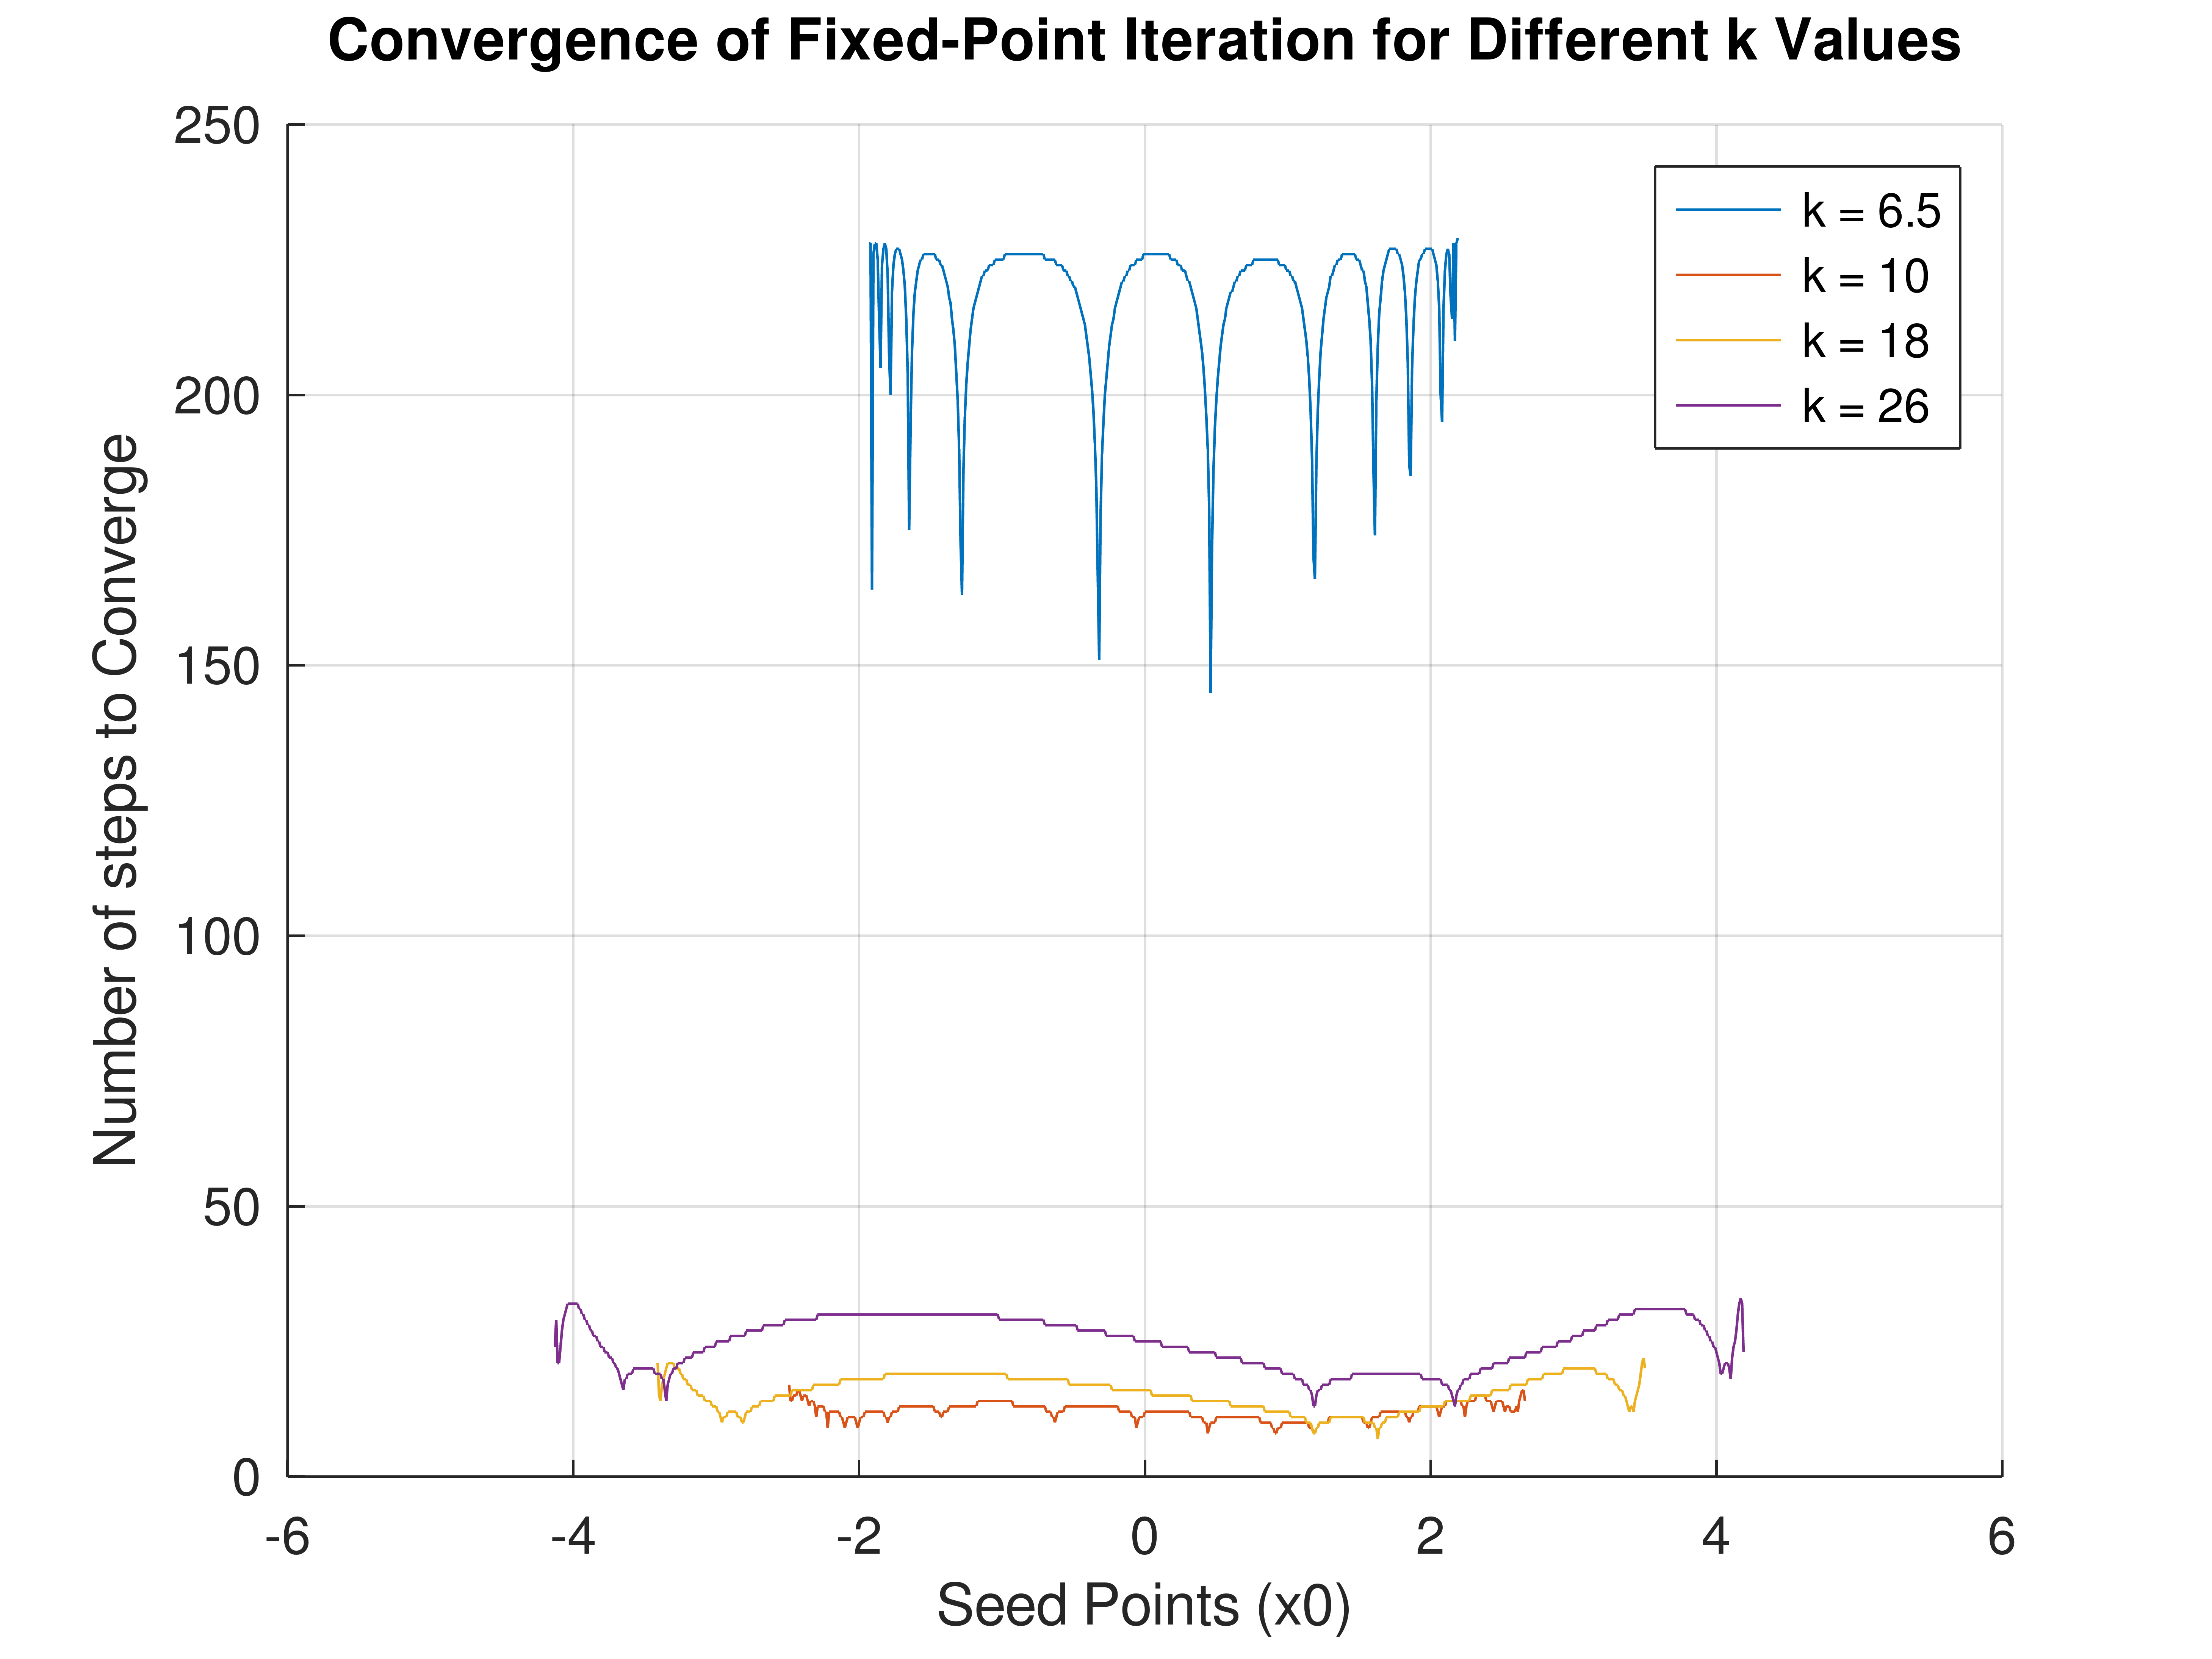
\includegraphics[width=1\textwidth]{/home/Baley/UTAS/org-roam/KME272-Assesment-1-2-Part1.png}
\end{center}
\subsection{2}
\label{sec:orgcbe3e70}
\begin{minted}[]{octave}
% Spliting the interval
R=1;
L=10;
SubInterval = 0:0.1:R;
% Using the intermediate value theorem
for i = 1:length(SubInterval)-1
    % f(SubInterval(i),R,L)
    % f(SubInterval(i+1),R,L)
    if f(SubInterval(i),R,L) > 0 && f(SubInterval(i+1),R,L) < 0
        % the interval contains the root
        Interval = [SubInterval(i), SubInterval(i+1)];
    end
        if f(SubInterval(i),R,L) < 0 && f(SubInterval(i+1),R,L) > 0
        % the interval contains the root
        Interval = [SubInterval(i), SubInterval(i+1)];
    end
end
a=Interval(1);
b=Interval(2);
fprintf("Both root finding methods will begin on the interval [%f,%f]\n",a,b)
fprintf("------------------------------------------------------------\n",a,b)
fprintf("The bisection method\n")
step = 1;
tol = 10^-6;
while true
    c = (a+b)/2;
    if f(a,R,L) * f(c,R,L) < 0
        b=c;
    else
        a=c;
    end
    epsilon = abs(f(c,R,L));
    if step > 2 && epsilon < tol
        break;
    end
    step = step +1;
    lastc = c;
    fprintf("steps = %i, epsilon = %f, c = %f\n",step,epsilon,c)
end
fprintf("------------------------------------------------------------\n",a,b)
fprintf("The regula-falsi method\n")
a=Interval(1);
b=Interval(2);
step = 1;
while true
    c=a-f(a,R,L)*((b-a)/(f(b,R,L)-f(a,R,L)));
    epsilon = abs(f(c,R,L));
    fprintf("steps = %i, epsilon = %f, c = %f\n",step,epsilon,c)
    if epsilon <= tol
        break
    else
        % Check which interval the root is in
        if f(b,R,L)*f(c,R,L) < 0
            a=c;
        else
            b=c;
        end
    end
    step = step + 1;
end
fprintf("------------------------------------------------------------\n",a,b)

function retval = f(h,R,L)
    Vmax=L*(R^2*(pi/2 - asin(0/R)) - 0*sqrt(R^2-0^2)); % Max occurs when h = 0
    retval= L*(R^2*(pi/2 - asin(h/R)) - h*sqrt(R^2-h^2)) - 0.9*Vmax;
end
\end{minted}

\phantomsection
\label{}
\begin{verbatim}
Both root finding methods will begin on the interval [0.000000,0.100000]
------------------------------------------------------------
The bisection method
steps = 2, epsilon = 0.571213, c = 0.050000
steps = 3, epsilon = 0.072204, c = 0.075000
steps = 4, epsilon = 0.176968, c = 0.087500
steps = 5, epsilon = 0.052414, c = 0.081250
steps = 6, epsilon = 0.009887, c = 0.078125
steps = 7, epsilon = 0.021265, c = 0.079688
steps = 8, epsilon = 0.005690, c = 0.078906
steps = 9, epsilon = 0.002099, c = 0.078516
steps = 10, epsilon = 0.001795, c = 0.078711
steps = 11, epsilon = 0.000152, c = 0.078613
steps = 12, epsilon = 0.000822, c = 0.078662
steps = 13, epsilon = 0.000335, c = 0.078638
steps = 14, epsilon = 0.000092, c = 0.078625
steps = 15, epsilon = 0.000030, c = 0.078619
steps = 16, epsilon = 0.000031, c = 0.078622
------------------------------------------------------------
The regula-falsi method
steps = 1, epsilon = 0.001002, c = 0.078671
steps = 2, epsilon = 0.000002, c = 0.078621
steps = 3, epsilon = 0.000000, c = 0.078621
------------------------------------------------------------
\end{verbatim}
\end{document}
